\subsection{PIMS Notification Module}
This module is responsible for sending email/SMS notifications to a patient. This email/text message could be a reminder to a patient about follow up visits to the doctor. \par 

\subsubsection{Scope}
The scope is shown in the use case diagram below: \par
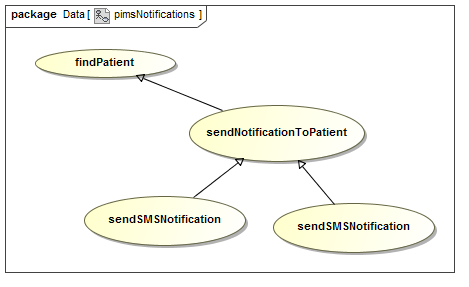
\includegraphics[width=0.75\linewidth]{./Graphics/pimsNotification/pimsNotifications}

\subsubsection{Use cases}
\begin{description}
	\item{\textbf{findPatient -- priority: nice-to-have}}
	This use case is to cater for the retrieval of a patient ID/name form the database so as to obtain the contact details of the patient, if any.
	\begin{description}
		\item{\textbf{Service Contract}} The service contract for findPatient is shown below.
		\begin{figure}[h!]
			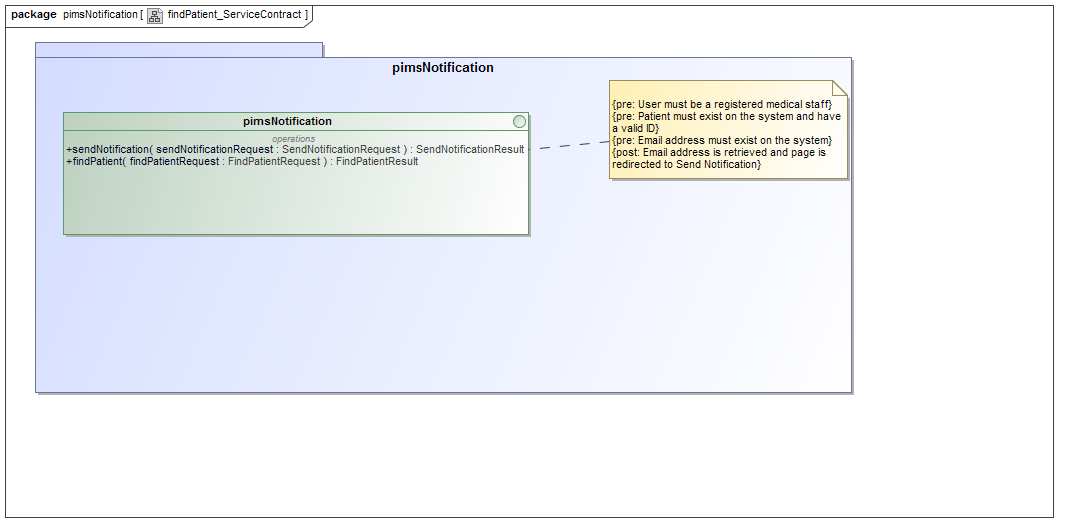
\includegraphics[width=\linewidth]{./Graphics/pimsNotification/findPatient_ServiceContract}
		\end{figure}
	\end{description}	
	
	\item{\textbf{sendSMSNotification -- priority: nice-to-have}}
	This use case is to cater for the sending of a follow-up notification message via SMS depending on whether or not the patient has a cellphone number that is stored on the system.
	\item{\textbf{sendEmailNotification -- priority: nice-to-have}}
	This use case is to cater for the sending of a follow-up notification message via E-mail depending on whether or not the patient has an email address that is stored on the system.
	
	\begin{description}
		\item{\textbf{Service Contract}} The service contract for sendSMSNotification and  sendEmailNotification is shown below.
		\begin{figure}[h!]
			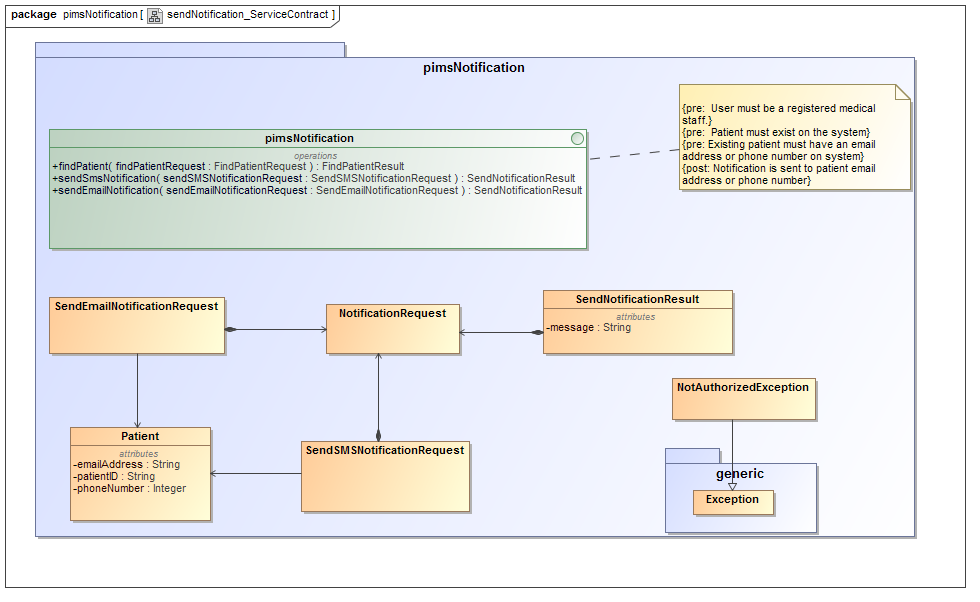
\includegraphics[width=\linewidth]{./Graphics/pimsNotification/sendNotificatioServiceContract}
		\end{figure}
	\end{description}		
	
\end{description}